\section{Electrical Impedance Tomography}

Most EIT systems consist of: 
a current source to inject a current between two electrodes;
a system to measure differential voltages between pairs of electrodes; and
electrodes, applied to the body surface.
This section further discusses each of these aspects of EIT 
and introduces concepts of image acquisition and reconstruction.


\subsection{EIT Measurements}
A ``frame'' of EIT data consists of a series of measurements made on an array
of electrodes placed around
a region of interest. This thesis focuses on measurements of the thorax. 

\subsubsection{Electrodes} \label{sec:electrodes}

EIT recordings are made using several types of electrodes. 
Both polarizable and non-polarizable
electrode types are used;
silver-silver chloride electrodes are often applied directly to the body,
and stainless steel, brass, textile and rubber electrodes have also 
been used and are sometimes 
integrated into electrode belts. 
The polarization of EIT electrodes is 
not significant at the frequencies (>20 kHz) that are typically used
\parencite{adler_electrical_2017}.

When making measurements with EIT systems, there is very little current flowing
through non-injecting electrodes due to the high impedance of the 
integrated voltmeter~\parencite{holder_electrical_2004}.
For this reason, the effects of the electrode-body impedance 
are minimal on electrodes that are not injecting current. Measurements that 
are largely affected by this impedance on injecting electrodes typically have a
phase shift and are often removed before reconstruction. 

Changing contact impedance has a large effect on EIT measurements 
can be influenced by changes in posture or pressure on electrodes 
\parencite{coulombe_parametric_2005}.
Contact impedance is often improved on electrodes by adding a
conductive gel \parencite{waldmann_performance_2017}, but it can decrease 
over long measurements as the gel dries \parencite{lozano_errors_1995}. 

\subsubsection{Current Injection and Voltage Measurement}
To calculate impedance, three main considerations must be made with regard to the 
injected current: the frequency, amplitude and injection pattern. 

Low frequency currents will 
preferentially pass around cells through the extracellular
fluid, due to the high capacitive component of the cell 
membrane~\parencite{foster_whole-body_1996}, whereas high frequency currents will be 
more affected by the capacitive 
component~\parencite{holder_electrical_2004}. 
Since EIT requires a linear relationship between the measured voltages and 
tissue impedance to produce valid reconstructions,
it is important to select frequencies of less than 1 MHz to ensure that cell 
and neural membrane is not the dominant factor in the impedance 
measurements~\parencite{barber_applied_1984}.
Impedance measurements below 100 kHz have shown to be primarily resistive (real) on lung
tissue~\parencite{witsoe_electrical_1967}, and most EIT systems use
frequencies between 10 kHz and 1 Mhz~\parencite{holder_electrical_2004}.

The selection of current amplitudes is primarily selected based on 
considerations to patient safety \parencite{adler_electrical_2017}.
The guideline defined by IEC 60601-1 
\parencite{international_electrotechnical_commission_iec_2021}, set a limit 
of 10 mA on current across all electrodes at 100 kHz, and lower limits 
at lower frequencies. 
For EIT, frequencies between 20--200 kHz are often used with 
an injected current
between 1--5 mA.
In order to meet the safety
guidelines at low frequencies,
when injecting sinusoidal currents it is also important to use complete current cycles 
so that DC currents are not applied to the body \parencite{adler_electrical_2017}.
When using internal electrodes, there are additional safety considerations that limit
current amplitudes. Depending on the proximity to the heart, for clinical use 
it may be required to not inject current on internal electrodes. They can still be used
to make measurements. 

The pattern of current injection and voltage measurement is commonly referred to in EIT 
as the stimulation and measurement pattern. Typically a current is injected between two electrodes
while the resulting voltages are measured between adjacent pairs. The two most common injection 
patterns are ``adjacent'', and ``skip 4''. Examples of these measurement patterns are shown in 
\fref{fig:stim_meas_bkgnd} on a 16-electrode system. The terms adjacent and skip 4 describe 
the space between pairs of injecting or measurement electrodes. 
Regardless of the pattern, a frame of EIT data is generated in the same way. 
Current is injected between a pair of electrodes as voltage is measured between all 
remaining pairs, then current is injected between the next pair of electrodes and
voltages are measured again. This results in voltage measurements on each electrode 
pair for every current injection. For a 16-electrode system, this results in 
256 measurements in each frame. For a 32-electrode system, there are 1024. As mentioned in 
\fref{sec:electrodes}, voltage measurements made on the stimulating electrodes
are often removed resulting in 208 measurements per frame on a 16-electrode system, and 928 measurements per frame on a 32-electrode system.  

\begin{figure}[H]
    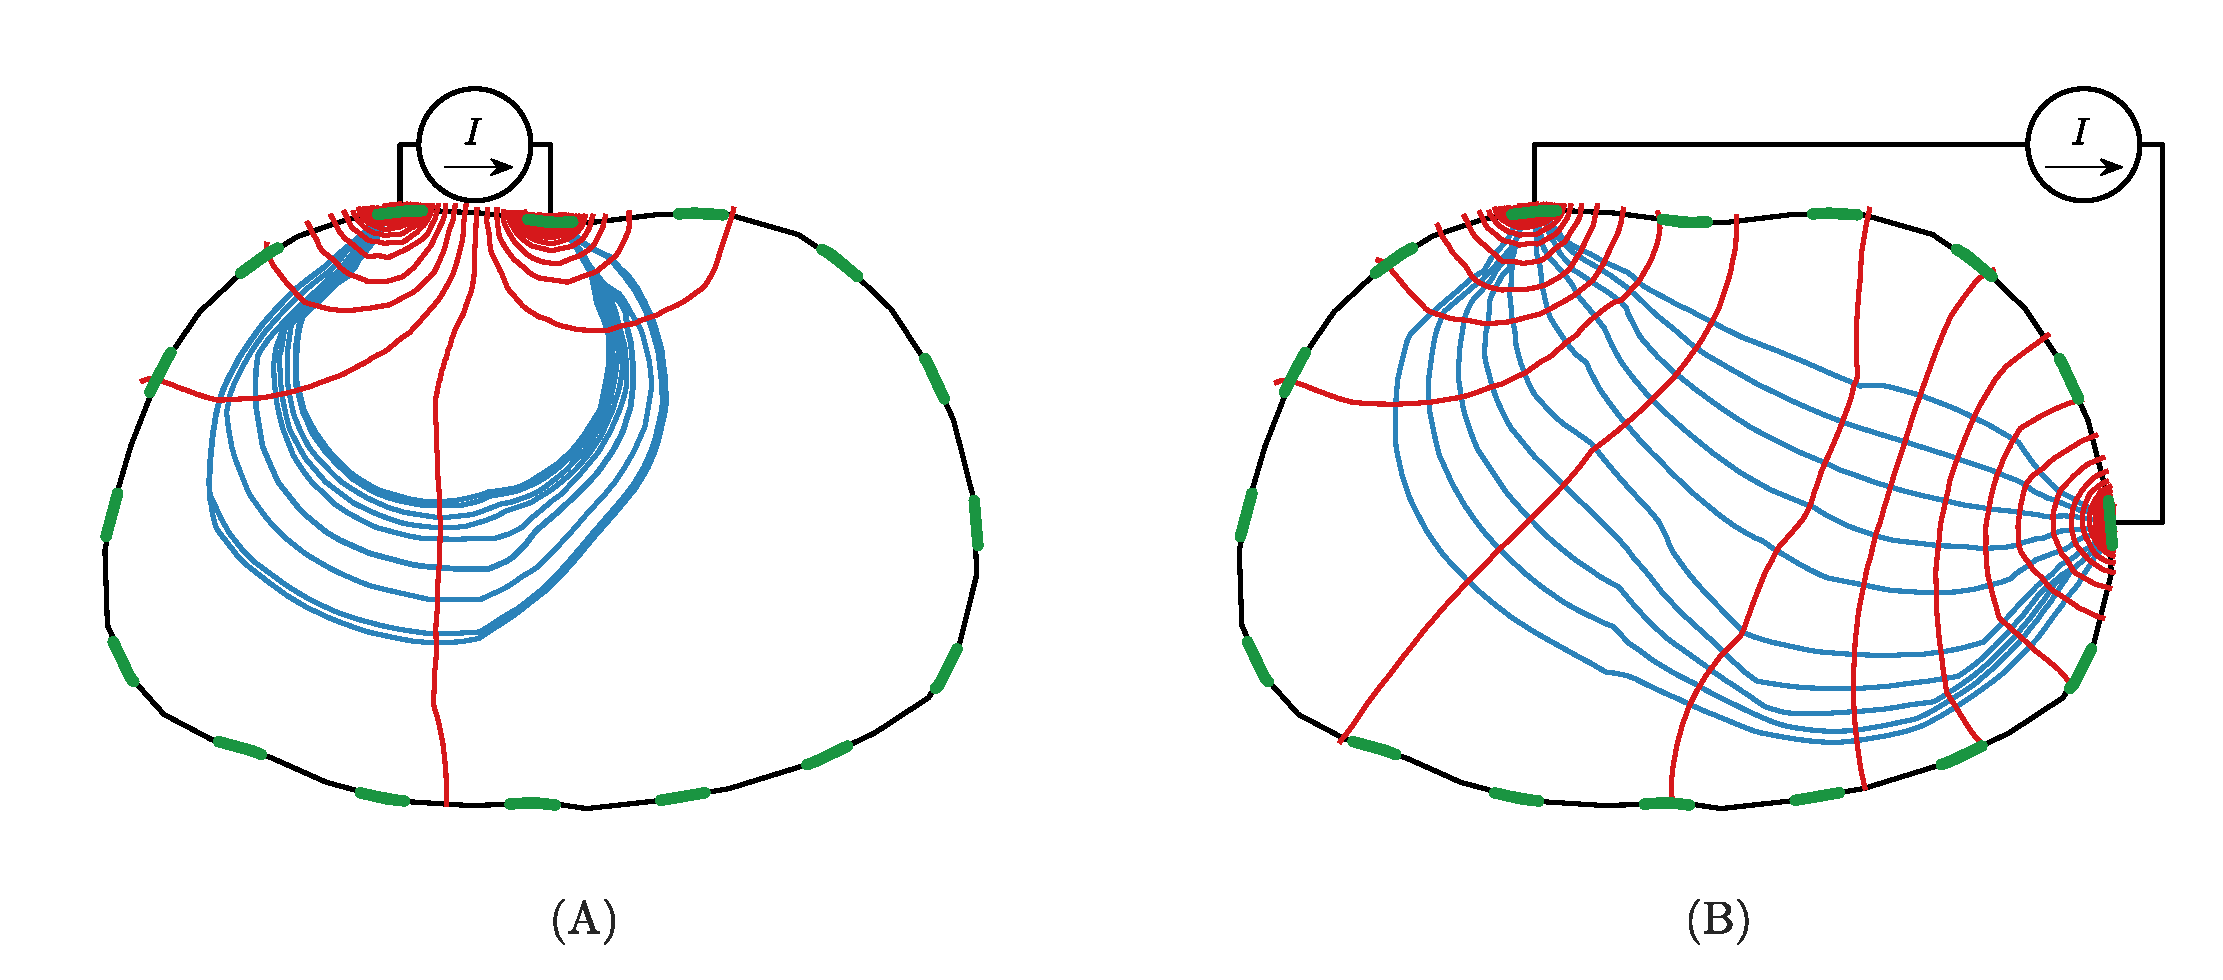
\includegraphics[width=\textwidth]{chapter2-background/imgs/common_stim_meas_patterns.pdf}
    \caption[Adjacent and ``skip 4'' stimulation patterns]{\label{fig:stim_meas_bkgnd} 
    Two common stimulation patterns are simulated on a simple human model shown in 
    \fref{fig:cur_equip_line}. Injected current is shown in blue and the resulting equipotential 
    lines are shown in red.
    (A) An example of an adjacent stimulation pattern. Current is injected between 
    pairs of adjacent electrodes. For each current injection voltage is 
    measured between all sequential pairs. 
    (B) An example of the ``skip 4'' injection pattern. Current is injected between every
    5\textsuperscript{th} electrode, skipping 4 between the injecting electrodes. 
    During each current injection, voltage measurements are made using the same skip 4 
    pattern between each of the 16 electrodes and their corresponding pair. 
    A single frame of data is generated by all measurements made for each possible injection
    pattern. For 16 electrodes, this results in 256 measurements.}
 \end{figure}


\subsection{Imaging Techniques}
There are several challenges that make absolute EIT imaging difficult. 
The differences in tissue impedances are subtle relative to artefacts introduced 
by unknown boundary locations and electrode 
positions~\parencite{adler_why_2015,adler_electrical_2017,nissinen_compensation_2009}. 
EIT is instead typically used to reconstruct impedance changes between two points in time.

Time difference EIT is sensitive to the movement of fluid within the body 
and is well suited to image functional activity, such as 
the inflation of the lungs 
and the flow of blood.
Time-difference EIT is also much more stable in the presence of errors that remain 
constant, such as incorrectly modelled boundary and electrode 
locations~\parencite{brown_electrical_2003}.
Frequency difference EIT is also possible based on the different impedance response 
of tissue types to changing frequencies. Frequency difference uses 
two or more different frequencies and calculates an image based on the change in electrical properties.
Most frequencies used to differentiate between different tissue types are at high frequencies 
where current starts to flow across the cell membranes. 
These high frequencies are out of the range of most current EIT systems, and 
frequency changes due to different lower frequencies are limited~\parencite{adler_electrical_2017}.
This thesis uses time-difference EIT to image changes in movement and fluid volumes in the thorax.

\subsection{Forward Problem} \label{sec:fwd}
In simulations, there is a model with known geometry and impedance and we wish to solve for the 
voltage at the electrodes, due to a stimulation current. 
This is called the forward problem. 
A model used to calculate a solution for the forward problem is called a forward 
model. 

This problem is well-posed, and can be solved analytically on simple, regular geometries. 
For the forward solution, Maxwell's formulation of Faraday's Law is required:
\begin{equation} \label{eq:farad}
\nabla \times \vec{E} = -\frac{\partial}{\partial t} \vec{B}
\end{equation}
and Ampere's Law: 
\begin{equation} \label{eq:amp}
\nabla \times \vec{H} = \vec{J} + \frac{\partial}{\partial t} \vec{D}.
\end{equation}

To set up the solution we first assume that the current used for EIT is sufficiently low 
frequency relative to the scale of interest that we can use a 
quasistatic approximation of Maxwell's equations \parencite{larsson_electromagnetics_2007}. 
Under this assumption the derivative components of \fref{eq:farad} and \fref{eq:amp}
can be set to zero giving:
\begin{equation}
\nabla \times \vec{E} = 0
\end{equation}
and
\begin{equation} \label{eq:amp2}
\nabla \times \vec{H} = \vec{J}.
\end{equation}
In this static case, the electric field due to a potential can be described by 
\begin{equation} \label{eq:field}
	\vec{E} = -\nabla\vec{u}.
\end{equation}

Finally, we require Ohm's Law, describing the relationship between the current density,
conductivity and electric field:
\begin{equation} \label{eq:ohm}
	\vec{J} = \sigma \vec{E}.
\end{equation}

Using the magnetic field identity for the divergence of curl 
($ \nabla \cdot (\nabla \times \vec{H}) = 0 $) with \fref{eq:amp2}, produces:
\begin{equation} \label{eq:mid1}
	\nabla \cdot \vec{J} = 0.
\end{equation}
Combining \fref{eq:mid1} with Ohm's Law (\fref{eq:ohm}) gives: 
\begin{equation} \label{eq:mid2}
	\nabla \cdot (\sigma \vec{E}) = 0.
\end{equation}
And finally, using \fref{eq:field} relating the electric field and potential 
yields: 
\begin{equation}
	\nabla \cdot \sigma \nabla \vec{u} = 0
\end{equation}
Which gives the relationship between a conductivity distribution and the resulting 
potential. 


The current density on the boundary is given by:
\begin{equation} \label{eq:cur_den}
	j_n = -\vec{J} \cdot \vec{n}  = \sigma \nabla \vec{u} \cdot \vec{n}.
\end{equation}
Where $\vec{n}$ is a unit vector normal to the boundary. \Fref{eq:cur_den} cannot be 
used to specify current density at the boundary in EIT where the current density is not 
uniform \parencite{somersalo_existence_1992}. Instead
we require a formulation that gives current density on injecting electrodes 
and no current density on the rest of the boundary.
\citeauthorandyear{somersalo_existence_1992} give 
a formulation of a complete electrode model for the voltage on $L$ electrodes ($E$)
where the voltage measured on each electrode ($U$) is constant. 
\begin{equation} \label{eq:comp_elec}
	u + z_l (\sigma \nabla u \cdot \vec{n}) = U_l ~~~~~ \text{on} ~~ E_l, ~~~~ l= 1,2,\cdot\cdot\cdot,L.
\end{equation}
The impedance of each electrode contact ($z$) is also typically treated as a constant over the surface of 
an electrode \parencite{somersalo_existence_1992}.
This complete electrode model has been shown 
to predict voltage accurately \parencite{somersalo_existence_1992}.

\subsection{Discretization and the Finite Element Method}
For EIT, analytic solutions are possible for simple geometries, but in a majority of cases
numerical methods are required. 
One of the primary discretization techniques is the finite element method \acrshort{fem}
where the domain is divided into a number of smaller elements. 
An element is
triangular in 2D and tetrahedral in 3D. 
The collection of nodes, and elements making up a larger model is commonly called a mesh. 
Each line connecting two nodes of a mesh can be visualized as a resistor,
used to model the conductivity of an object.

To accurateatly solve numerical problems using the FEM, it is vital to accurately represent 
spatial information. \citeauthorandyear{boyle_impact_2011} show that incorrectly modelling 
the boundary and electrodes can result in distorted images. 
Especially in brain EIT, great care is taken to minimize errors in the forward model 
\parencite{aristovich_method_2014,malone_multifrequency_2014}, 
as small errors
in modelling have been shown to give large errors in the reconstructed 
images \parencite{kolehmainen_assessment_1997}. 

\subsection{Inverse Problem} \label{sec:inv_prob}
To reconstruct images, we must solve for impedance distribution from known voltage measurements. 
This is known as the inverse problem. 
The ability to reconstruct impedance distributions from a known voltage distribution is challenging 
and relies on the assumption that the relationship between voltage and conductivity is 
linear \parencite{barber_applied_1984}.
Unlike the forward problem, due to the small number of electrodes 
relative to the large number of internal elements the inverse problem is
ill-posed \parencite{holder_electrical_2004}.

The sensitivity of EIT is often represented by a jacobian matrix, $\mathbf{J}$,
which gives the change in measurement relative to another factor. To reconstruct 
a conductivity distribution, a conductivity jacobian, $\mathbf{J}_C$, is used
which links the change 
in boundary voltage measurements to the change in impedance. It can be represented by 
\begin{equation} \label{eq:jacobian_c}
	[\mathbf{J}_C]_{ij} = \frac{\partial U_i}{\partial \sigma_j}. 
\end{equation}
The jacobian gives the relationship between the conductivity of each voxel and the resulting
measurements \parencite{holder_electrical_2004}.
In practice the jacobian can be calculated using the adjoint 
field \parencite{vauhkonen_three-dimensional_1999}. 

\subsubsection{Regularization}
The sensitivity of measurements to changes is vastly different throughout the model. 
Near electrodes, where the current density is high, there is high sensitivity to conductivity 
changes but there is limited sensitivity away from the electrodes. This contributes 
to the ill-posed nature of the inverse problem \parencite{holder_electrical_2004}.
To overcome this regularization must be used to stabilize reconstruction. 
Regularization imposes restrictions on a minimization problem to ensure a unique solution.
In EIT, some typical regularization techniques include the maximum \emph{a priori} approach
\parencite{adler_electrical_1996}, Tikhonov regularization \parencite{vauhkonen_tikhonov_1998},
and singular value decomposition \parencite{ostebee_rank-deficient_1998}.

\subsubsection{Image Reconstruction}
The standard linear formulation \parencite{holder_electrical_2004} 
to solve for the conductivity change in each 
voxel ($\Delta \mathbf{\hat{\sigma}}$) for a given set of difference measurements ($\mathbf{b}$) is
\begin{equation}
	\Delta \mathbf{\hat{\sigma}} = \mathbf{J}^T \mathbf{\Sigma}_n 
	(\mathbf{J} \mathbf{\Sigma}_p \mathbf{J}^T + \mathbf{\Sigma}_p)^{-1} \mathbf{b}. 
\end{equation}
Where $\mathbf{\Sigma}_n$ and $\mathbf{\Sigma}_p$ are covariance matricies that 
incorporate \emph{a priori} information. 
$\mathbf{\Sigma}_n$ representes covarience in the data space and weights noise 
contribution to reconstructed images, and
$\mathbf{\Sigma}_n$ representes covariance in the image space, and 
controls regularization \parencite{adler_electrical_1996}.
The term $ \mathbf{J}^T  \mathbf{\Sigma}_n
(\mathbf{J} \mathbf{\Sigma}_p \mathbf{J}^T + \mathbf{\Sigma}_p)^{-1} $ is also called the 
reconstruction matrix and can be represented by the term
$\mathbf{R}$, since after initial calculation it typically remains constant for a given model. 
Conductivity distributions can be solved using the reconstruction matrix using the equation:

\begin{equation} \label{eq:rm_solve}
	\Delta \mathbf{\hat{\sigma}} = \mathbf{R} \mathbf{b}. 
\end{equation}

There are several techniques used to calculate error weighting and prior information represented by 
$\mathbf{W}$,
such as the NOSER algorithm \parencite{cheney_noser_1990}. There are also 
techniques that have been specifically designed 
to compensate for the limitations and characteristics of EIT systems 
such as GREIT \parencite{adler_greit_2009}.

\subsubsection{Image Reconstruction with GREIT}

GREIT (Graz consensus Reconstruction algorithm for EIT) is 
a consensus algorithm that is used to reconstruct EIT images 
according to limitations and characteristics of typical EIT systems 
\parencite{adler_greit_2009}. 
The reconstruction matrix calculated with GREIT depends on the
forward model, noise model and the desired performance metrics.
GREIT uses a forward model that models electrodes using 
the complete electrode model discussed in \fref{sec:fwd}.
The forward model has information regarding the stimulation measurement pattern,
body geometry, and electrodes.

GREIT constructs a set of training images using a small (less than 5\% of the model diameter) 
conductive target in the 
forward model. A training set consists of images of a conductive object
placed at many (100--500) locations within the model. 
A noise model consisting of a Gaussian estimate of measurement noise, 
and measurements with electrode motion noise is also generated. 

Training targets are blurred so that their diameter increases to 20\% of 
the model diameter, but the position remains constant. 
This is used as the desired image for a training target. 
The weighting relative to noise and other performance metrics 
is set to minimize reconstruction errors between the training target and ideal image. 
The weights are set based on the radius of the training image to penalize
changes outside the desired image radius and minimize shape deformation
and ringing artefact. The weighting can also be adjusted to meet specific performance 
characteristics of interest. A description of all performance characteristics that 
can be specified is found by \citeauthorandyear{adler_greit_2009}. 
When training the GREIT algorithm, weighting is also set to increase uniformity 
of the resolution in the reconstructed image. Some resolution near the electrode is 
lost, but weighting helps to ensure that targets reconstruct to the same size throughout the model.

To calculate a reconstruction matrix ($\mathbf{R}$), error ($\epsilon$)
is minimized over all training targets ($k$) with respect to the 
weighting parameters ($\mathbf{w}^{(k)}$),
measurements ($\mathbf{b}$), and the desired images ($\mathbf{\tilde{x}}$).
\begin{equation} \label{eq:greit_min}
	\epsilon^2 = \sum_{k} \|\mathbf{\tilde{x}}^{(k)}
    - \mathbf{Rb}^{(k)}\|^{2}_{\mathbf{w}^{(k)}}
\end{equation}
To minimize the equation for error, the derivative of $\epsilon^2$ with respect to the reconstruction 
matrix is set to 0.
\begin{equation} 
	\epsilon^2 = \sum_{k} \|\mathbf{\tilde{x}}^{(k)}
    - \mathbf{Rb}^{(k)}\|^{2}_{\mathbf{W}^{(k)}}
\end{equation}
%\citeauthorandyear{petersen_matrix_2008} present the identity 
%Using the identity 

\citeauthorandyear{grychtol_3d_2016} show that \fref{eq:greit_min} can 
be rearranged to solve for the reconstruction matrix
as:
\begin{equation} 
	\mathbf{R} = \mathbf{D}  
	\mathbf{\Sigma}_p \mathbf{J}^T(\mathbf{J}  
	 \mathbf{\Sigma}_p  \mathbf{J}^T + 
	 \lambda \mathbf{\Sigma}_n)^{-1}
\end{equation}
Where $\mathbf{D}$ is the desired image metric from all training images,
$\mathbf{\Sigma}_p$  is the effective covariance of all training targets after weighting with 
$\mathbf{W}$, and 
$\mathbf{\Sigma}_n$ is the noise covariance. 
%It is assumed that the noise on each measurement is independant and not correlated to other measurements 
%which is not always true \parencite{adler_minimizing_2011}. 
%The calculated noise covarience matrix is assumed be 
This reconstruction method is widely used in EIT for both 2D and 3D electrode configurations 
and is shown to give even resolution throughout the image \parencite{adler_greit_2009}.

\subsection{Internal Electrodes}

While there have been some studies researching electrode placement for cardiac
imaging in 2D~\parencite{vonk_noordegraaf_improvement_1996} and 
3D electrode configurations~\parencite{graham_electrode_2007}, there has 
been little research into the application of internal electrodes. 
It has been shown that externally placed 3D electrode configurations
consisting of two electrode planes
can improve the sensitivity distribution and image quality~\parencite{grychtol_3d_2016},
but there is still limited sensitivity in the central-most regions 
of the chest.
The concept of using internal esophageal reference electrodes has been presented
previously
\parencite{pilkington_utilization_1989,schuessler_utility_1995}
as a method to improve internal sensitivity, and has shown
accuracy improvements of up to 30\% for small 
targets \parencite{pilkington_utilization_1989}.
Recent simulations in 2D have shown an increase in reconstruction 
accuracy, amplitude response, position error, and resolution
\parencite{nasehi_tehrani_modelling_2012,nasehi_tehrani_evaluation_2012}

A clinical evaluation of EIT found that the amplitude of cardiosynchronous signals 
in EIT measurements was 6 times larger when placing 2 of 16 total electrodes in 
either the esophagus or trachea, but found that reconstructions 
in an animal model were not obviously improved in all cases \parencite{czaplik_application_2014}.
A recent review highlighted the use of internal electrodes to monitor cardiac radiofrequency
ablation; investigate the possible noise sources; and 
stated the need for analysis of the effect of motion on the 
internal electrodes
\parencite{nguyen_electrical_2020}.

Despite several promising simulation results using internal electrodes, the clinical advantage
has not been realized. 
*****
but internal electrodes have not been widely used clinically. 
**** Conversations with collegues *** at least 2 sentences.
While studies show an increased sensitivity to cardiosynchronous
EIT signals, the source of these signals is not clear, and the impact of movement 
on the internal electrodes is not known. 

\section{Summary}
EIT has potential to be used as a tool for continuous perfusion monitoring at the bedside,
but is limited by low sensitivity to cardiosynchronous signal. 
Accurate modelling and 
the use of internal electrodes have been proposed as techniques to 
increase the sensitivity of EIT in specific regions, 
but it is not clear how much these might improve perfusion imaging. 
We also examine the effect of internal electrode movement and potential
methods to correct these errors. 
Improving sensitivity to cardiosynchronous signals with EIT could enable 
better isolation of the perfusion related signal from other factors, and 
improve the use of EIT for cardiovascular monitoring. 


%\subsubsection{3D Reconstruction}
%The majority of EIT measurements are done with a single ring of external electrodes but 
%in practice, electrical current cannot  be confined to a single plane
%and using a two dimensional electrode configuration can significantly
%impact the capabilities of \acrshort{eit}~\parencite{Rabbani1991}.
%The use of 3D electrode configurations in \acrshort{eit}
%was introduced in 1996~\parencite{Metherall1996} to overcome the 
%inherent limitations of 2D measurements, but it is still not widely used today.
%It is thought this is due to the increased complexity of 3D images
%and the subsequent analysis~\parencite{Grychtol2019}.
%
%Several studies have shown that there may be several advantages to using an internal
%electrode in \acrshort{eit} recordings; 
%Measurements with an internal electrode have been 
%shown to reconstruct images equally as well as configurations with 
%twice as many external electrodes~\parencite{Schuessler1995},
%and have shown an increase in sensitivity in a central region 
%of interest~\parencite{Kwon2013,Czaplik2014,Farooq2014}.

%\subsubsection{Inverse Source localization (time permitting)}









% TODO in the thesis go into absolute imaging vs time difference imaging in depth here!!!

%\section{Perfusion monitoring}
%\subsection{Contrast agent injection}
%\subsection{Frequency Filtering}
%
%
%Monitoring lung ventilation is one of the most
%established clinical uses of 
%\acrshort{eit}, presented initially by Barber and Brown~\parencite{Barber1984}.
%EIT has also been used as a tool to monitor blood 
%perfusion~\parencite{Brown1992} and hemodynamic parameters such as 
%cardiac output~\parencite{Braun2018} and blood pressure~\parencite{Sola2011,Proenca2017}. 
%While the spatial resolution of \acrshort{eit} is much lower than 
%intermittent imaging techniques such as \acrfull{ct} or \acrfull{mri},
%\acrshort{eit} can have a high temporal resolution enabling continuous or frequent 
%monitoring without concerns regarding radiation exposure.
%This thesis focuses on time difference EIT for thoracic hemodynamic imaging and monitoring applications. 
%
%
%%\section{Aortic flow monitoring}
%%
%%Continuous bedside monitoring appears to be one of the most
%%promising future applications of \acrshort{eit} due to the high 
%%temporal resolution, and concerns with other imaging modalities 
%%and the associated radiation 
%%exposure. 
%%
%%%There are several hemodynamic parameters that are widely used to asses cardiovascular 
%%%health. One of the most used is cardiac output (CO), the amount of blood pumped through the
%%%heart in one minute.
%%%The two most used method is
%%%thermodilution using a Swan-Ganz catheter~\parencite{Khalil1963} in the pulmonary artery, 
%%%which determines CO by injecting a solution with a known temperature and 
%%%measuring the temperature change~\parencite{ReuterDaniel2010}. This method is considered the gold standard of 
%%%CO monitoring~\parencite{Joosten2017}.
%%
%%Another potential use of EIT is to replace invasive monitoring techniques
%%such as catheterized measurements of pulmonary arterial pressure.
%%Recent studies have evaluated EIT as a method of determining 
%%pulmonary arterial pressure using pulse wave velocity in the 
%%descending aorta in 2D~\parencite{Braun2018a,Proenca2017,Proenca2016}.
%%EIT was a used in conjunction with ECG signals and shown to have a high correlation
%%with pulmonary arterial pressure values from from Doppler echocardiography~\parencite{Proenca2016}.
%%
%%An analysis of hemodynamic measures using EIT found that measures of stroke 
%%volume and pulmonary arterial pressure are sensitive to electrode placement and
%%interference from pulmonary signals~\parencite{Braun2018a}. 
%%The solution proposed in this document uses an arrangement of internal electrodes placed in the 
%%esophagus adjacent to the aorta to increase the sensitivity to changes and improve detection 
%%accuracy and elimination of pulmonary signals.
%%
%%Improving tracking and imaging of the aorta is also important because it
%%has additional clinical uses: it  can be used as a physiological landmark to identify
%%the back of the lungs, and can be used to continuously monitor blood pressure by
%%calculating the pulse transit time. 
%
%
%
%\acrshort{eit} has been used clinically to monitor lung perfusion 
%in an animal model~\parencite{Leonhardt2012,Nguyen2012}, and it is theorized that 
%the use of an internal electrode for increased sensitivity may allow for 
%imaging of blood flow in the aorta. 
%There is great interest in monitoring cardiac parameters
%using \acrshort{eit} to determine \acrfull{sv}~\parencite{Proenca2017,Braun2018}, and increased
%sensitivity close to the heart also has the potential to improve
%these measures.
%
%While there have been some studies researching electrode placement for cardiac
%imaging in 2D~\parencite{Noordegraaf1996} and 
%3D electrode configurations~\parencite{Graham2007}, there has 
%been little research into determining the optimal 3D external electrode configurations
%for imaging the heart and aorta. 
%
%Additionally when using alternate electrode configurations the current injection and 
%measurement patterns must also be investigated. It has been suggested that  an internal electrode
%in 2D
%should not be used for current injection in asymmetrical models
%as the reconstruction performance deteriorates~\parencite{NasehiTehrani2012}. 
%It is unclear 
%to what degree injection patterns affect the resulting sensitivity when
%internal electrodes and alternate electrode arrangements are used in 3D.
%
%This work aims to investigate internal and 
%external electrode configurations for use in imaging blood movement 
%in the thorax, and develop techniques to extract measures of 
%aortic flow and lung perfusion from these reconstructions.
%
%%\subsubsection{3D \acrshort{eit} image reconstruction}
%%It has been shown that when the continuous boundary voltages of a surface are
%%known, there is a unique solution to the inverse problem used to calculate internal 
%%conductivity~\parencite{Calderon2006},
%%but EIT uses discrete measurements of boundary voltage 
%%and there is no unique solution. 
%%
%%In order to reconstruct EIT images prior information and smoothing 
%%must be used to obtain a solution. There are several reconstruction methods used in 
%%EIT including Tikhonov regularization~\parencite{Tikhonov1977} and 
%%standardized methods for EIT such as GREIT~\parencite{Adler2009}.
%%A version of GREIT for 3D reconstructions~\parencite{Grychtol2016}
%%is used in this work.